%!TEX TS-program = xelatex
%!TEX encoding = UTF-8 Unicode

\documentclass{IMTA-report}

\begin{document}
\pagenumbering{arabic}
% the front matter
\documenttype{Rapport de Stage de fin d'étude}
%Images
\schoollogo{
\includegraphics[width=0.3\textwidth]{figures/IMTAlogo.jpg}}
\enterpriselogo{
\includegraphics[width=0.4\textwidth]{figures/edgemind_logo.png}}
\decologo{
\includegraphics[width=0.7\textwidth]{figures/deco_cover_page.png}}
% Details du rapport
% REM RD : Bidouille pour mettre un sous titre juste après le titre et non après le texte "Rapport
% de Stage"
\title{Modélisation d’une chaîne de traitements de données pour le diagnostic/pronostic des
pannes \\ \vspace{10pt} \Large Application à la recommandation des actions de maintenance}
\author{Thomas BAZAILLE}

% sur le diplome
\degree{Diplome Titre}
\field{Titre du rapport}
\degreeyear{2020}
\degreemonth{Août}

% sur l'école
\department{\ }
\university{Institut Mines Télécom Atlantique}
\universitycity{Nantes}
\universitystate{Loire Atlantique, FRANCE}

% sur l'entreprise
\enterprisedepartment{Morbihan}
\enterprise{EdgeMind}
\enterprisecity{Vannes}
\enterprisestate{FRANCE}

\maketitle
\copyrightpage
\abstractpage
\tableofcontents
%\authorlist
\listoffigures

\onehalfspacing

% REM RD : Suggestion de forme qui irait bien pour ton rapport à mon avis.
% - Tu as 5 chapitres qui ressemblent plus à des "parties", i.e. des éléments assez indépendants
% - => Je te suggère donc de faire 3 parties :
%      1. Prensentation entreprise
%      2. Projet
%         - Tu peux à mon avis fusionner 2.1, 2.2, 2.3, 3.1 dans un chapitre "Mise en contexte"
%         - Ensuite tu transormes tes sections 3.x 2<=x<=9 en Chapitre
%      3. Apport du projet (en y incluant la conclusion)
% Tu peux faire des parties en LaTeX avec la commande \part{Nom de la partie} cf. exemple dans projet.tex

% include each chapter...
%\documentclass[a4paper]{article}
%\usepackage[ampersand]{easylist}
%\usepackage{parskip}
%\usepackage{graphicx}
%\begin{document}

\chapter{Présentation de la société EdgeMind}
\section{Présentation}

EdgeMind a été créée le 13 janvier 2014 par Roland Donat et Thomas  Friedlhuber sous la forme d’une SAS. Le 1er septembre 2016, ils sont rejoints par Vincent Leblond. Ces trois personnes constituent à la fois l’équipe dirigeante de la société et les experts techniques.

\begin{easylist}
\ListProperties(Hide=100, Hang=true, Progressive=3ex, Style*=--)
& ~Roland Donat : Président ;
& ~Thomas Friedlhuber : Directeur Général ;
& ~Vincent Leblond : Directeur commercial et projets.
\end{easylist}

L’actionnariat est détenu à 100\% par ces trois personnes physiques, salariées de la société et dont l’activité professionnelle est entièrement consacrée au développement de EdgeMind.

\section{Ressources humaines}

\begin{minipage}{0.7\textwidth}

À ce jour, EdgeMind se compose de 10 personnes localisées à Vannes, Nantes et Paris :
\begin{easylist}
\ListProperties(Hide=100, Hang=true, Progressive=3ex, Style*=--)
& ~7 salariés en CDI (dont l’équipe dirigeante) ;
& ~1 salariés en contrat d’apprentissage ;
& ~2 stagiaires de fin d’études niveau BAC+5.
\end{easylist}

\end{minipage}%
%
\begin{minipage}{0.4\textwidth}
\begin{center}
	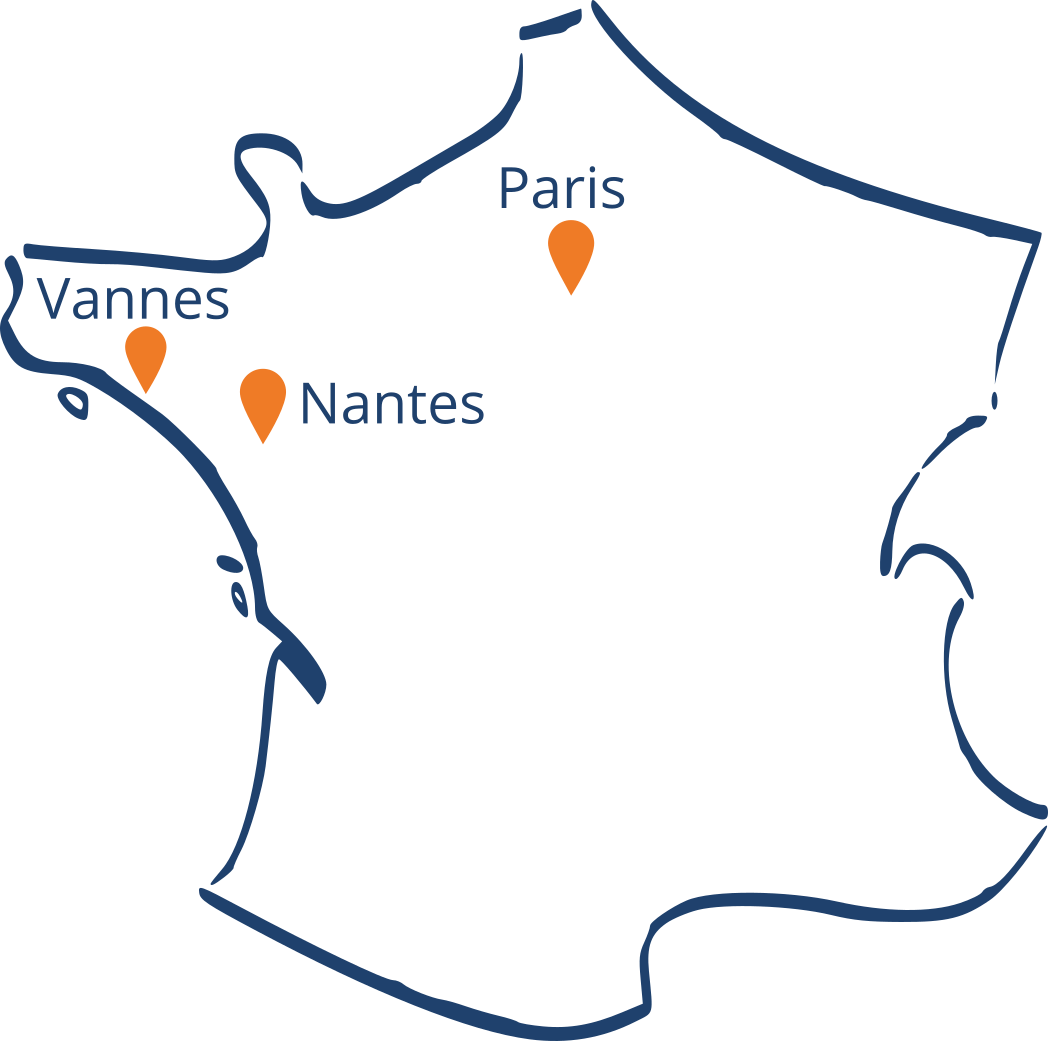
\includegraphics[scale=0.1]{figures/mini_france.png}
    \label{img:g}
\end{center}
\end{minipage}

Les compétences techniques du personnel couvrent :
\begin{easylist}
\ListProperties(Hide=100, Hang=true, Progressive=3ex, Style*=--)
& ~l’informatique scientifique ;
& ~la data science, machine learning et data visualisation ;
& ~la simulation multi-agent et la simulation de systèmes complexes ;
& ~l’analyse et la maîtrise des risques industriels ;
& ~la conception et la planification de systèmes de transport ;
& ~la recherche opérationnelle et l’optimisation ;
& ~le développement informatique desktop ;
& ~le développement informatique web ;
& ~la réalisation d’études et de prestations de conseil.
\end{easylist}

\section{Valeurs}

EdgeMind promeut et défend plusieurs valeurs dans ses relations commerciales et partenariales :
\begin{easylist}
\ListProperties(Hide=100, Hang=true, Progressive=3ex, Style*=--)
& ~Transparence ;
& ~Innovation et recherche scientifique ;
& ~Écoute des besoins métiers ;
& ~Relation de confiance ;
& ~Indépendance de ses activités.
\end{easylist}

\section{Activités, partenaires R\&D et clients}

EdgeMind est une société indépendante spécialisée dans l’innovation scientifique. Son activité repose sur la commercialisation de prestations et d’outils informatiques pour l’aide à la décision et l’optimisation de la performance opérationnelle. Ses secteurs d’activités privilégiés sont les transports, l’énergie et les territoires.

Les activités de EdgeMind couvrent les domaines de la maintenance prédictive, la maîtrise des risques industriels, la simulation des systèmes de transports et la valorisation des données métiers.

Les partenaires R\&D et les clients sont listés ci-dessous :


\includegraphics[scale=0.6]{figures/clients_logo.png}

\section{Activités de recherche et innovation}

EdgeMind consacre plus de 50\% de son activité à la Recherche et Développement afin de constamment faire évoluer ses solutions et répondre aux besoins de ses clients. Nous cherchons également à débloquer les verrous scientifiques rencontrés lors de nos projets en nous appuyant sur nos liens avec des chercheurs issus d’instituts de recherche académique ou de l’industrie. Il est à noter que la société EdgeMind bénéficie du statut de Jeune Entreprise Innovante.

En 2018, EdgeMind a décidé d’investir avec ses fonds propres à hauteur de 160 K€ dans un projet de recherche partenarial au sein de l’Institut de Recherche Technologique System X. Ce projet sera réalisé sur une durée de 4 ans. Les grands objectifs de ce projet sont les suivants :
\begin{easylist}
\ListProperties(Hide=100, Hang=true, Progressive=3ex, Style*=--)
& ~spécifier et structurer les données opérationnelles afin d’identifier et formaliser les sources de données nécessaires à l’analyse des stratégies de maintenance ;
& ~améliorer le diagnostic des défaillances à partir de données complexes et hétérogènes ;
& ~modéliser les processus de maintenance prévisionnelle et déployer la chaîne d’outils associés sur des cas tests industriels ;
& ~élaborer une méthodologie générale pour la simulation et l’évaluation technico-économique des politiques de maintenance;
& ~développer des algorithmes d’optimisation globale des stratégies de maintenance en incluant les processus de soutien logistique associés.
\end{easylist}

Les partenaires du projet sont des industriels du secteur de l’énergie, de l’aéronautique et du transport.



\includegraphics[scale=0.5]{figures/clients_logo2.png}


\includegraphics[scale=0.5]{figures/clients_logo2bis.png}
%\end{document}
\begin{savequote}[75mm] 
This is some random quote to start off the chapter.
\qauthor{Firstname lastname} 
\end{savequote}

\chapter{Mise en contexte}

\section{Origine du projet et enjeux}

\subsection{Contexte de l'étude}

Sur le réseau francilien, Paris et sa banlieue, la RATP exploite et maintient près de 5 000 bus. La maintenance est réalisée dans un peu plus de 25 centres bus répartis sur l’ensemble du territoire des lignes exploitées.
Le département MRB en charge de la maintenance cherche à améliorer continuellement l’efficacité des opérations de maintenance. Un axe d’amélioration porte sur l’élaboration de recommandations visant à assister les mainteneurs dans leurs opérations de maintenance.
Le département MRB souhaite également mutualiser l’expertise des mainteneurs. En effet, les mainteneurs des centres bus interviennent sur des matériels analogues sans pouvoir aisément bénéficier de l’expérience de leurs collègues situés sur les autres centres bus.
Par ailleurs, le contexte du matériel bus évolue fortement avec l’acquisition de nombreux véhicules électriques. Cette situation conduit à une accélération du renouvellement du parc de véhicules. Pour assurer la bonne exploitation des véhicules, les mainteneurs doivent ainsi rapidement monter en expertise sur ces nouveaux véhicules.
En 2019, EdgeMind répond à une demande de la RATP qui cherche à pouvoir effectuer efficacement un diagnostic de pannes de ses bus.


\subsection{Objectif du projet}

Le projet vise à développer un outil de recommandation des opérations de maintenance sur les bus. Le développement de l’outil repose sur la valorisation des données de GMAO (Gestion de Maintenance Assistée par Ordinateur) disponible au sein du département MRB.

Le projet se décompose de la manière suivante :
\begin{easylist}
\ListProperties(Hide=100, Hang=true, Progressive=3ex, Style*=--)
& ~exploitation et traitement des données ;
& ~modélisation des recommandations ;
& ~développement d’une application métier pour les utilisateurs finaux ;
& ~expérimentation de l’outils sur plusieurs mois.
\end{easylist}

C’est dans ce contexte que EdgeMind a ensuite lancé le développement en R\&D d’un outil générique de machine learning spécifique au domaine de la maintenance afin d’enrichir ses propres outils de machine learning. L’étude de la RATP sera alors un cas d’usage permettant les tests de ces développements.


\section{Problématique et mission}

La problématique de ce stage de fin d’études est de créer une chaîne de traitement orientée machine learning pour faire du pronostic/diagnostic spécifiquement dans le domaine de la maintenance.

Les différentes phases du projet à effectuer sont les suivantes:
\begin{easylist}
\ListProperties(Hide=100, Hang=true, Progressive=3ex, Style*=--)
& ~Création d’un module générique de préparation de données
& ~Ajout de différents type de modèle de machine learning (réseaux bayésiens, arbres de décisions (decision tree) , forêts aléatoires (random forests), réseaux de neurones, etc)
& ~Développement d’un module d’évaluation de performance d’un modèle donné
& ~Visualisation des indicateurs de performances
\end{easylist}

\section{Description des données GMAO Bus de la RATP}

Tout au long des développements, les tests seront effectués sur la base de données GMAO de la RATP. L’étude est un problème de classification supervisée. 

Les données de la base GMAO sont temporelles, i.e. les premières données sont les plus anciennes et les dernières données rentrées dans la base sont les plus récentes. Cela a son importance car il faudra prendre en compte dans les modèles que l’équipement matériel évolue très rapidement dans l’industrie, et cela influe donc forcément les types de maintenance à effectuer. Les problèmes liés à la maintenance en 2020 ne sont pas les mêmes qu’en 2010. Ainsi afin de bien prédire un type de maintenance, il faut s’intéresser aux données récentes.

Par ailleurs ces données contiennent un vocabulaire spécifique que nous allons détailler ici. Tout d’abord, lorsqu'une anomalie est détectée sur un bus, le conducteur émet un \textbf{signalement} afin de noter les caractéristiques de cette anomalie. Les caractéristiques sont enregistrées dans la base de donnée GMAO. Ensuite, un ordre de travail (\textbf{OT}) est émis suite à ce signalement, lequel aboutira ou non à un ordre de maintenance (\textbf{ODM}). L’objectif de l’étude est alors de prédire les ODM à effectuer à partir des données de signalement et des caractéristiques du bus en question.
\chapter{Modélisation et organisation du projet}
\clearpage
\section{Organisation du projet}

Les trois premières semaines du stage ont consisté à réaliser un état de l’art scientifique et technique sur les approches de modélisation probabiliste \cite{pradhan_knowledge_1994} \cite{dechter_bucket_1998} \cite{nielsen_bayesian_2009} et en particulier sur le formalisme des réseaux bayésiens et leurs applications  dans le domaine du diagnostic/pronostic de pannes. \cite{giurgiu_explainable_2019}\cite{noauthor_transparency_2019} \cite{chen_railway_2019}\cite{shi_fault_2006}\cite{zhang_fault_2017}\cite{cai_bayesian_2017}\cite{krishnamurthi_expert_1992}\cite{huang_probability_2008}\cite{chen-fu_chien_using_2002}\cite{han_universal_2008}

Une seconde phase de mise à niveau technique a permi de se familiariser avec  l’écosystème Python pour la \textit{data science}. En particulier, les librairies utilisées dans les implémentations sont Pandas pour le traitement de données, Pyagrum pour la modélisation de réseaux bayésiens, Scikit-learn pour les  méthodes usuelles de \textit{machine learning}, Pytest pour effectuer des tests unitaires et enfin Pydantic pour la structuration et la lisibilité du code. L’ensemble des développements est effectué sous gestion de versions avec le logiciel Git.

Durant le mois qui suit, une première version du module d’évaluation de performances et les premières visualisations ont été codées en appliquant les récentes connaissances acquises (en jaune sur la figure \ref{diagramme_gantt}).
Il s’ensuit une longue phase d’environ deux mois où le coeur du projet a été codé en se basant sur le framework déjà existant (en rouge sur le diagramme). En effet, EdgeMind avait déjà implémenté un début de structure de la chaîne de traitement.

Puis un mois a été accordé à l’ajout de mesures de performance spécifiques au pronostic, et à l’ajout d’un module de comparaison de performance (en bleu).

Enfin le projet s’est terminé par une phase de correction de bugs et de documentation afin de permettre la continuité du projet (en orange sur le diagramme).

% REM RD :
% - N'hésite pas à encapsuler tes figures dans un bloc "figure" pour avoir accès à des options de
% placement plus riche, cf. exemple ci-dessous.
\begin{figure}
  \centering
  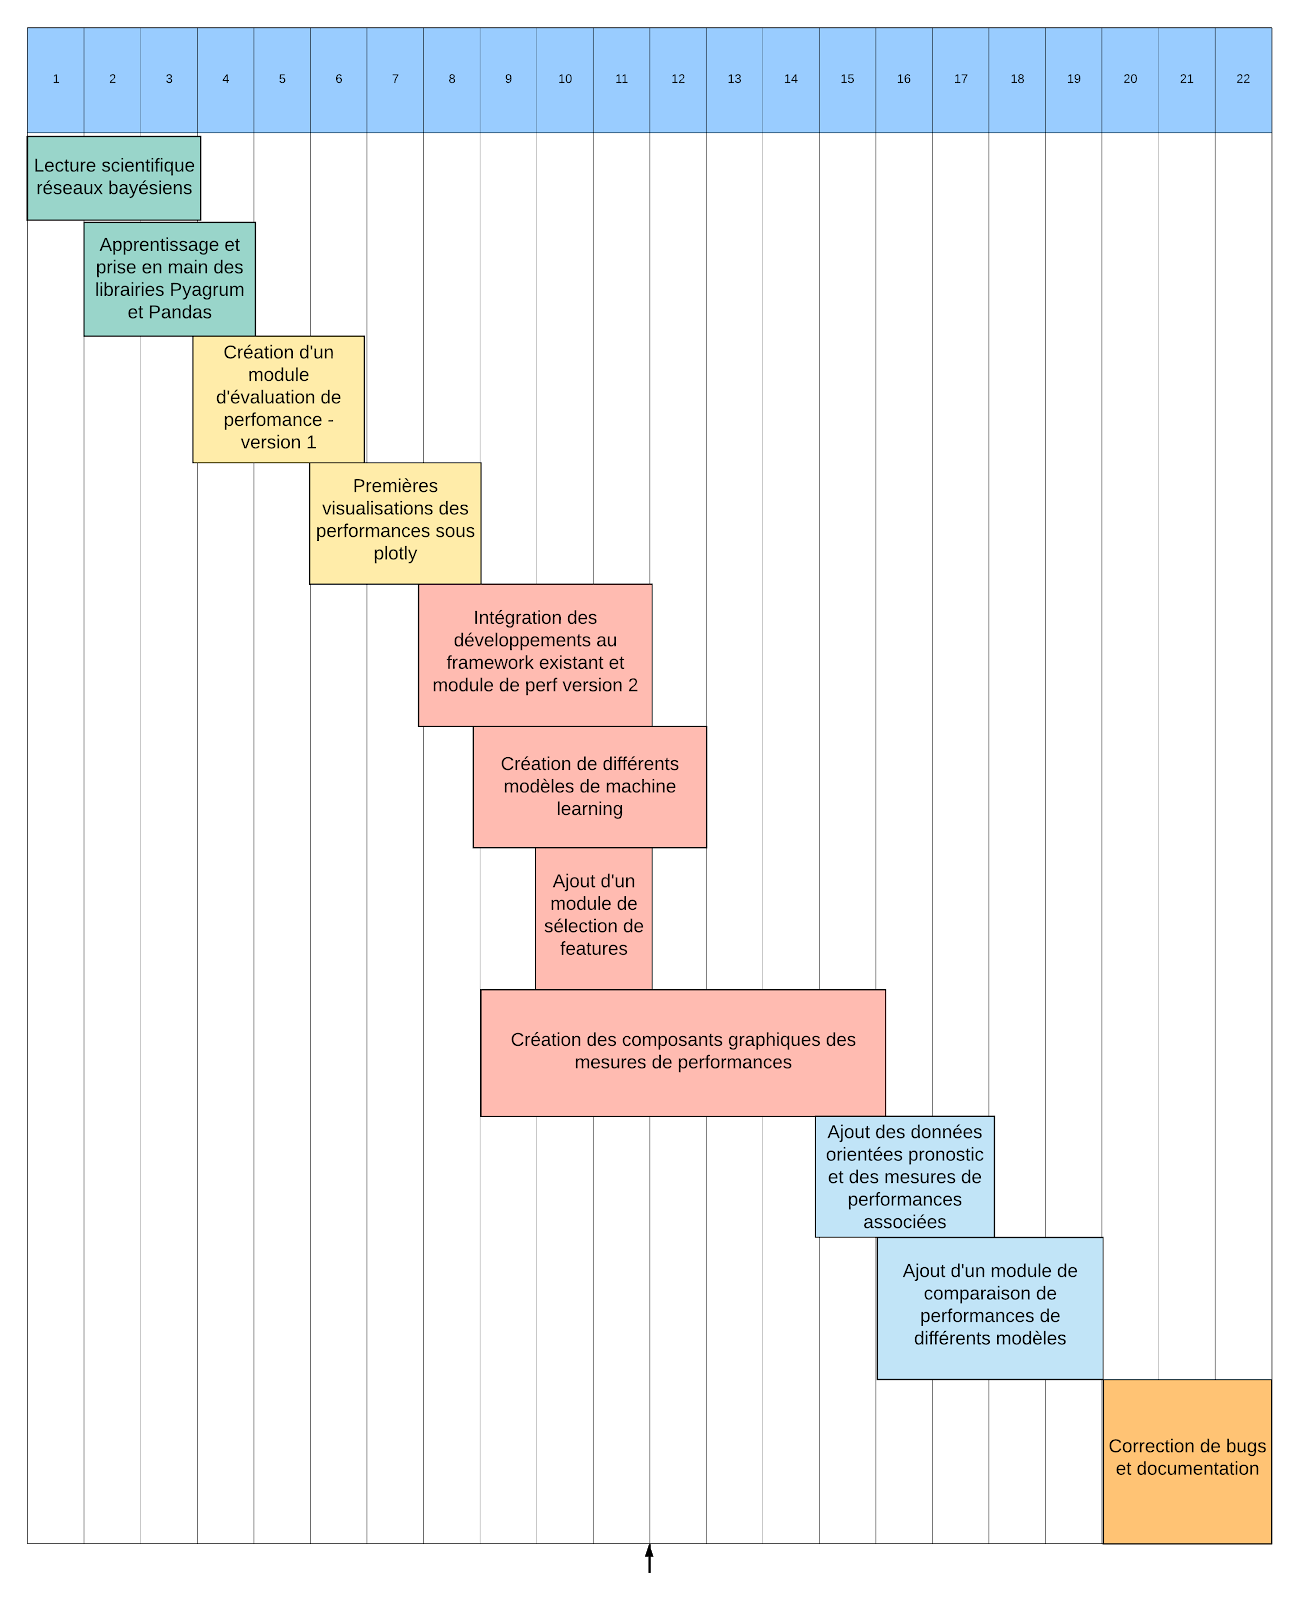
\includegraphics[width=1\textwidth]{figures/Rapport_GANTT.png}
  \captionof{figure}{Diagramme de GANTT}
  \label{diagramme_gantt}
\end{figure}

% Astuce pour afficher ton diagramme de gantt pas trop loin du texte
\clearpage

\section{Aperçu de la chaîne de diagnostic/pronostic}

% REM RD: Là, il faudrait un petit texte introductif à mon avis
La modélisation de la chaîne de traitement comporte les quatre modules présentés dans la section \ref{modules}. En voici le schéma par blocs :


\begin{center}
  % REM RD :
  % Tu peux utiliser la largeur de la page pour caler tes figures plus facilement
  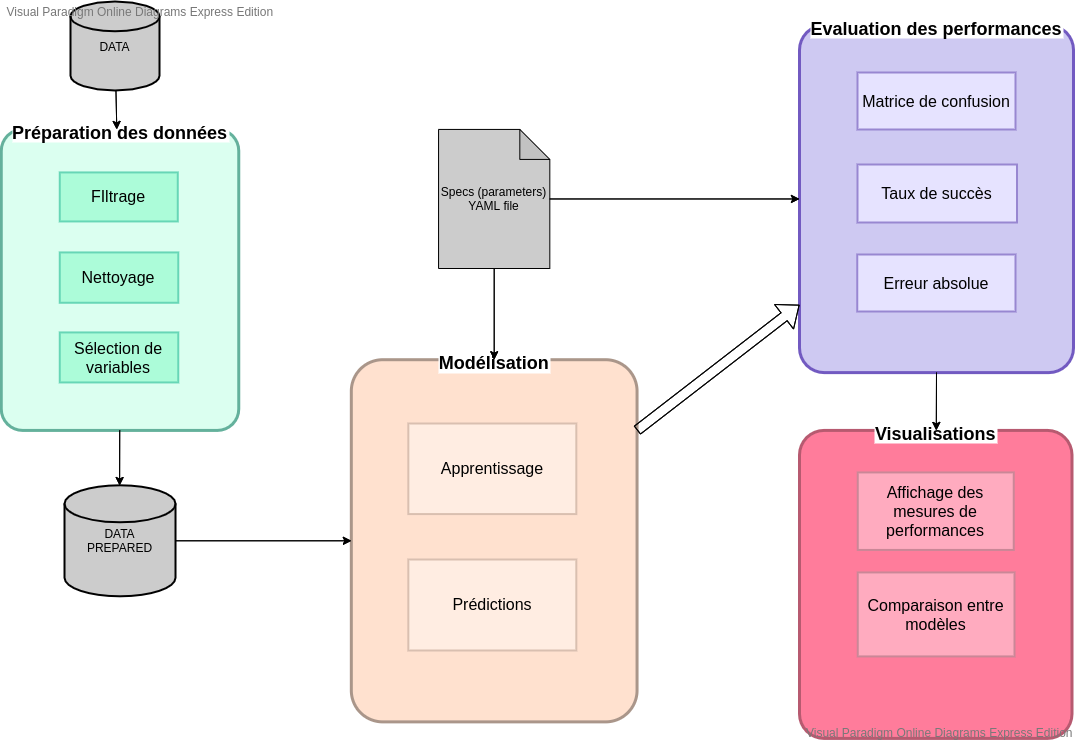
\includegraphics[width=1\textwidth]{figures/Bloc_diagram.png}
  \captionof{figure}{Diagramme par blocs}
  \label{bloc_diagramme}
\end{center}

\section{Préparation des données}
% REM RD : si tu choisis de faire des parties et donc de transformer cette section en chapitre, ça
% risque de faire un peu léger.
% À mon avis, tu peux faire inclure ce paragraphe dans le chapitre précédent où tu présente l'aperçu
% de la chaîne et expliquant rapidement cette phase de préparation de données.

\subsection{Filtrage}

Avant de mettre en oeuvre différents algorithmes de prédiction, il faut pouvoir assurer que les données sont conformes à ce que l’on souhaite. Plusieurs types d’action sont réalisées comme la mise en conformité des chaînes de caractère, le filtrage des données manquantes, la discrétisation des valeurs numériques pour certains algorithmes, etc.

Il est également possible de construire de nouvelles variables explicatives à partir des données pour améliorer les prédictions (\textit{feature engineering}).

\subsection{Sélection des variables}

Pour améliorer la précision des prédictions et pour accélérer la phase d’apprentissage, il peut être judicieux de se restreindre à un nombre limité de variables explicatives (ou \textit{features} en anglais), c’est ce qu’on appelle classiquement en \textit{machine learning} une méthode de réduction de la dimensionnalité. En effet, des redondances dans les données peuvent engendrer des problèmes au moment de l’apprentissage, comme le sur-apprentissage (ou \textit{overfitting} en anglais) par exemple.

Pour cela deux types de méthodes ont été implémentées : 
\begin{enumerate}
\item les méthodes de filtrage qui sélectionnent des variables indépendamment du modèle utilisé. Elles ne se basent que sur les corrélations entre les \textit{features} et les variables cibles. Leur principal avantage est qu’elles sont particulièrement efficace en terme de complexité temporelle.
\item les méthodes par encapsulation (\textit{wrapper method}) qui testent des sous-ensembles de \textit{features} sur le modèle, i.e. il faut faire un apprentissage du modèle pour chaque sous-ensemble que l’on veut tester. Ces méthodes sont plus précises mais elles sont beaucoup plus coûteuses en temps. Si on a $n$ variables et que l’on veut tester tous les sous-ensembles possibles, il faudrait faire $2^{n}$ phases d’apprentissage. La complexité étant exponentielle, on se limite en pratique à un nombre réduit de sous-ensembles à tester.
\end{enumerate}

Les deux méthodes de filtrage qui ont été ajoutées sont:
\begin{easylist}
\ListProperties(Hide=100, Hang=true, Progressive=3ex, Style*=--)
& ~FCBF (\textit{Fast Correlation-Based Filter}) \cite{fcbf_algorithm}
& ~ReliefF (une amélioration de l’algorithme Relief) \cite{Kononenko94estimatingattributes} 
\end{easylist}

La méthode d’encapsulation (\textit{wrapper method}) implémentée consiste quant à elle à tester l’impact de la suppression de chaque variable explicative, on a ainsi une complexité de l’ordre du nombre de variables.

\begin{center}
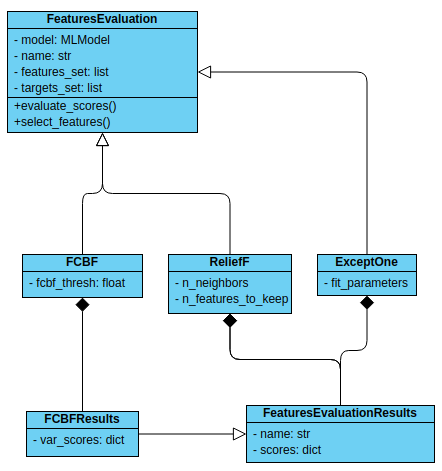
\includegraphics[width=0.8\textwidth]{figures/diagramme_classe_select.png}
\captionof{figure}{Diagramme de classe du module de sélection de variables}
\label{fig14}
\end{center}

\chapter{Modélisation des algorithmes de classification supervisée}
\clearpage
\section{Problématique}

La classification supervisée \cite{azencott2018introduction} peut être définie de la façon suivante: étant données $n$ observations $\lbrace\vec{x}^{\:i}\rbrace_{i=1,...,n}$ décrites dans un espace $\mathcal{X}$ et leurs étiquettes $\lbrace y^{\:i}\rbrace_{i=1,...,n}$ associées décrites dans un espace $\mathcal{Y}$, on cherche alors, à partir des données, une fonction $f:\mathcal{X}\rightarrow\mathcal{Y}$ telle que $\forall(\vec{x},y)\in \mathcal{X}\times\mathcal{Y},\quad f(\vec{x})\approx y$

\begin{center}
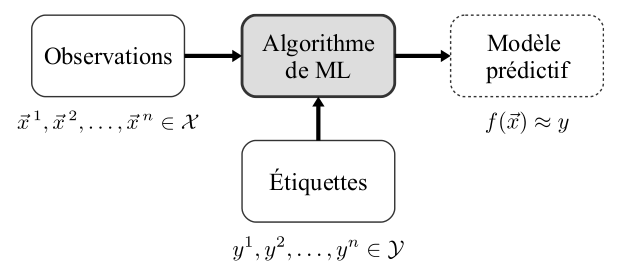
\includegraphics[width=0.8\textwidth]{figures/apprentissage_supervise.png}
\captionof{figure}{Apprentissage supervisé}
\label{fig3}
\end{center}

\section{Architecture du module de machine learning}

Afin de pouvoir garantir l’intégration de différents modèles de machine learning, une architecture de classes a été proposée et implémentée (cf. Figure \ref{diag_classe_ml})

\begin{center}
  % REM RD : N'hésite pas à agrandir tes diagrammes au max
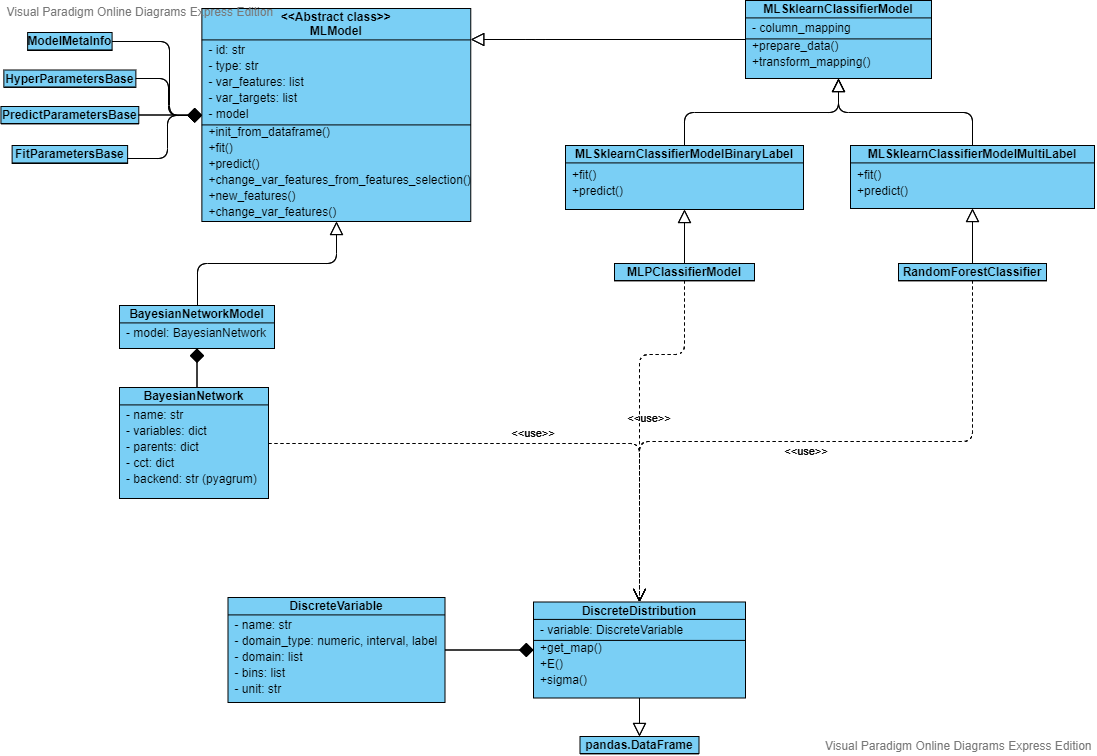
\includegraphics[width=1\textwidth]{figures/diagramme_classe_ml.png}
\captionof{figure}{Diagramme de classe des modèles de \textit{machine learning}}
\label{diag_classe_ml}
\end{center}

L'architecture proposée modélise une méthode de \textit{machine learning} sous forme d'une classe possédant :
\begin{easylist}
\ListProperties(Hide=100, Hang=true, Progressive=3ex, Style*=--)
& ~des hyperparamètres pour initialiser la classe (e.g. nombre de couche pour un réseau de neurones, etc)
& ~une méthode fit qui effectue l’apprentissage du modèle à partir d’un jeu de données d’entraînement
& ~une méthode predict qui renvoie le résultat des prédictions à partir d’un jeu de données de test. Cette fonction “predict” renvoie un objet \texttt{DiscreteDistribution}, qui est une sous-classe de la classe \texttt{pandas.DataFrame}, dans lequel chaque colonne correspond à chaque label de la variable cible et chaque ligne représente une ligne du jeu de test contenant les différentes probabilités de prédire chaque label.
\end{easylist}

\section{Exemple d'utilisation de la classe \texttt{MLModel}}

Imaginons que nous ayons le jeu de donnée suivant : 
\begin{easylist}
\ListProperties(Hide=100, Hang=true, Progressive=3ex, Style*=--)
& ~une variable à prédire “METEO” avec pour labels “SOLEIL”, “PLUIE”, “NUAGEUX”
% REM RD: on parle plutôt de variables explicatives
& ~deux features (ou variables caractéristiques) “TEMP” (pour température) et “HUM” (pour humidité)
\end{easylist}

Un jeu de données type aurait cette forme là par exemple:

\begin{center}
\begin{tabular}{cccc}
\rowcolor[RGB]{200, 200, 200}index & HUM & TEMP & METEO \\
\hline
1 & 50 & 18 & PLUIE \\
2 & 5 & 27 & SOLEIL \\
3 & 10 & 25 & SOLEIL \\
4 & 70 & 15 & NUAGEUX

\end{tabular}
\captionof{table}{Jeu de données}
\label{tab1}
\end{center}

L’utilisateur choisit un modèle ML et rentre ces données dans le modèle pour que s’effectuent la phase d’apprentissage suivie de la phase de prédiction.
Ces données sont alors divisées en jeu de test (index 3 et 4) et en jeu d’entraînement (index 1 et 2). On entraîne le modèle avec le jeu d’entraînement et on prédit à partir du jeu de test.

On aurait alors pour notre jeu de test de 2 lignes, une \texttt{DiscreteDistribution} de cette forme:

\begin{center}
\begin{tabular}{cccc}
\rowcolor[RGB]{200, 200, 200}index & SOLEIL & PLUIE & NUAGEUX \\
\hline
3 & 0.5 & 0.2 & 0.3 \\
4 & 0.3 & 0.3 & 0.4

\end{tabular}
\captionof{table}{\texttt{DiscreteDistribution}}
\label{tab2}
\end{center}

Il faut ensuite choisir comment classifier à partir d’une \texttt{DiscreteDistribution}. Une stratégie classique de classification consiste à prendre le MAP (\textit{maximum a posteriori}) de cette distribution.

Par exemple pour la ligne d'index 3 la prédiction la plus probable (i.e. le MAP) est “SOLEIL” et “NUAGEUX” pour la ligne d'index 4.

% REM RD: Titre un peu sec à mon avis.
% Il faudrait quelque chose du genre "Implémentation d'algorithmes de machine learning dans le
% framework" mais en plus cours :)
\chapter{Implémentation d'algorithmes ML}

Comme le montre la Figure \ref{diag_classe_ml}, trois modèles différents ont été implémentés. Un modèle regroupe différents algorithmes pour effectuer un apprentissage et des prédictions sur des données. Les deux algorithmes importants à implémenter dans chaque modèle sont donc la fonction d’apprentissage \textit{fit}  et la fonction de prédiction \textit{predict}.

% REM RD: Je reviens sur ma proposition ultérieure consistant à faire deux sous-sections par modèle
% décrit :
% 1. Présentation formelle de la technique avec explication et un chouille de théorie + exemple
% 2. Implémentation dans le framework
\clearpage
\section{Réseaux bayésiens}

% REM RD : Pour la biblio, utilise \cite{label} mais tu trouveras des tonnes d'aide sur le net pour ça.
Un réseau bayésien \cite{neapolitan_learning_2007} est un modèle graphique probabiliste représentant un ensemble de variables
aléatoires sous la forme d'un graphe orienté acyclique. Les noeuds de ce graphe correspondent aux
variables, tandis que les liens correspondent à des relations entre variables. Pour construire un
réseau bayésien, il faut donc définir les différentes variables et les tables de probabilités
conditionnelles pour chacune de ces variables sachant leurs parents dans le graphe. Si on a les variables aléatoires $(X_{i})_{i=1,...,n}$, alors la loi jointe du réseau s’écrit :
$$P(X_{1}, ...,X_{n})= \prod_{X \in (X_{1}, ...,X_{n})} P(X|pa(X))$$
où $pa(X)$ représente les parents immédiats de la variable aléatoire $X$ dans le graphe.

% REM RD: Sauf erreur de ma part, tu ne fais pas référence à la fig6 dans le texte. Si tu donnes un
% exemple, il faut que tu le détailles un minimum (quitte à ce que ce soit fait en annexe).
\begin{center}
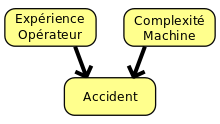
\includegraphics[width=0.6\textwidth]{figures/exemple_RB.png}
\captionof{figure}{Exemple de modélisation graphique d’un réseau bayésien}
\label{fig6}
\end{center}

Par exemple dans la Figure \ref{fig6}, la variable Accident a deux parents, Expérience Opérateur et Complexité Machine.

Le classe \textbf{BayesianNetworkModel} (Figure \ref{fig4}) permet de construire de tels réseaux bayésiens. Les calculs probabilistes (inférence) sont effectués par  la librairie \texttt{Python} \texttt{PyAgrum} dans la version actuelle des développements. Toutefois l’architecture offre une abstraction vis-à-vis de la méthode de calculs utilisées laissant ainsi la possibilité d’utiliser d’autres librairies de calcul ou d’implémenter ses propres algorithmes.
\clearpage
\section{Réseaux de neurones}
% REM RD: Il manque la partie où on explique ce qu'est un RN
Un réseau de neurones informatiques s'inspire du fonctionnement du cerveau humain en tentant de recréer la complexité de ce dernier. Il est constitué de plusieurs couches de neurones reliés entre eux. 

Le modèle choisi pour le réseau de neurone est la classe \textbf{MLPClassifier} (\textit{multi layer perceptron}) de la librairie scikit-learn. 

La construction de ce réseau est la suivante:
\begin{easylist}
\ListProperties(Hide=100, Hang=true, Progressive=3ex, Style*=--)
& ~une couche \textit{input} contenant les valeurs des différentes \textit{features}. Cette couche ne prend en entrée que des valeurs numériques. Si les données des \textit{features} sont des chaînes de caractères, il faut modifier ces valeurs en données numériques au préalable.
& ~un certain nombre de couche cachées contenant chacune le nombre de neurones que l’on souhaite
& ~une couche de sortie, qui correspond à la variable cible, contenant autant de neurones que cette variable cible n’a de labels. En sortie, chaque neurone se verra attribuer un score entre 0 et 1 selon la fonction d’activation \textit{softmax}. On peut interpréter ce score en terme de probabilité. Ainsi on peut considérer que cette sortie est une \texttt{DiscreteDistribution}.
\end{easylist}

\begin{center}
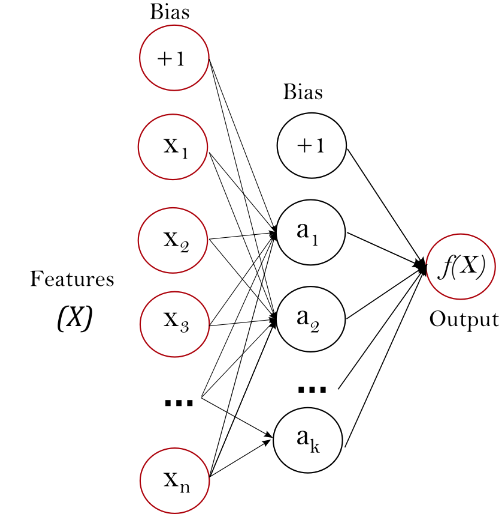
\includegraphics[width=0.5\textwidth]{figures/exemple_MLP.png}
\captionof{figure}{Exemple de MLP contenant une couche cachée}
\label{fig7}
\end{center}

\section{Forêts aléatoires}

Une forêt aléatoire est un algorithme combinant plusieurs arbres de décisions afin d’effectuer des prédictions plus fines qu’un arbre de décision seul. Le modèle choisi est la classe \textbf{RandomForestClassifier} de la librairie scikit-learn.

\begin{center}
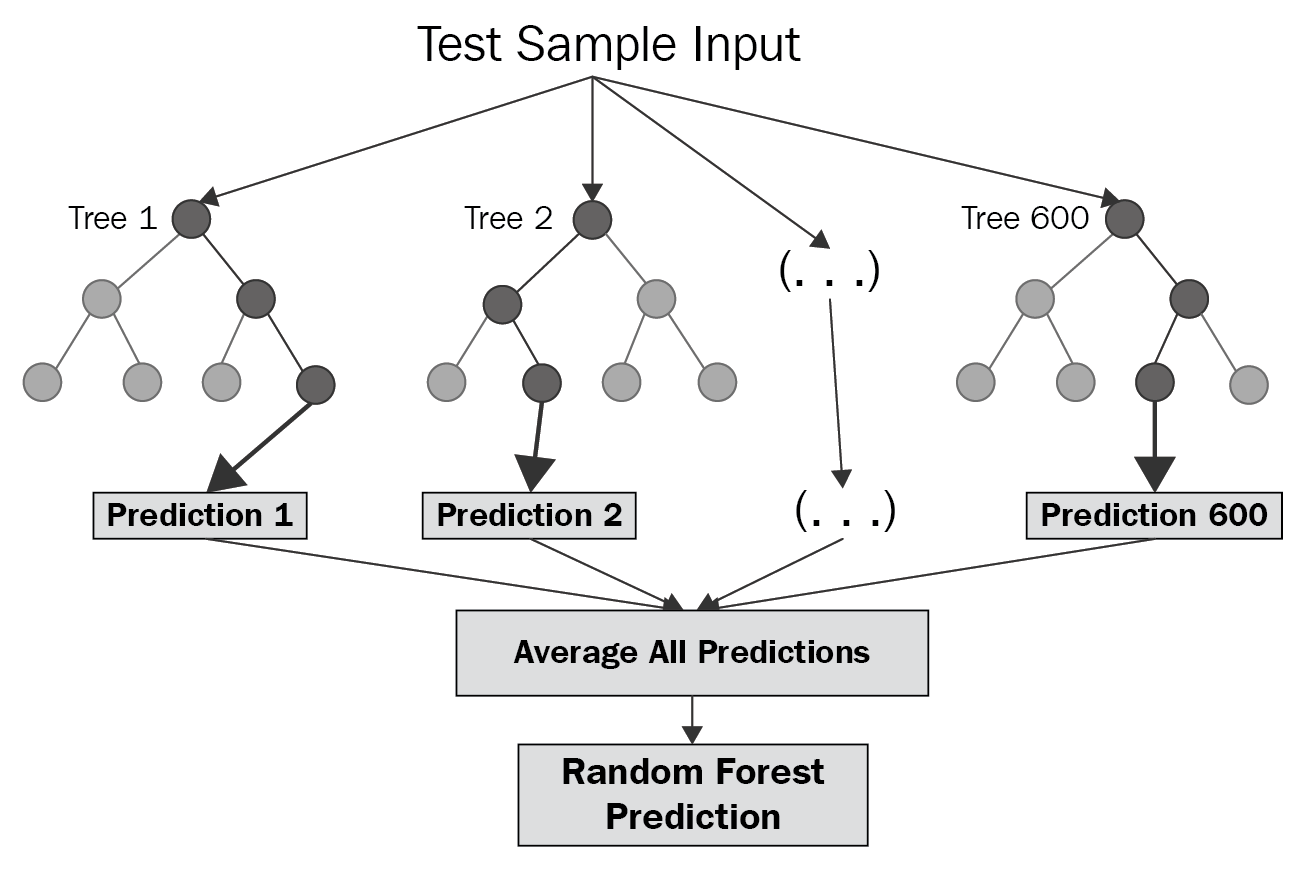
\includegraphics[width=0.8\textwidth]{figures/exemple_RF.png}
\captionof{figure}{Schéma forêt aléatoire}
\label{fig8}
\end{center}

% REM RD: Il manque la partie où on explique l'implémentation de RF

% REM RD: Utilise plutôt "framework de modélisation" à la place de "chaîne de traitements"
% La chaîne de traitements correspond à l'ensemble des briques de traitements allant du nettoyage
% des données à l'évaluation des perf en passant par la modélisation.
\section{Adaptation au \textit{framework} de modélisation}

% REM RD: Partie à relire et adapter légèrement pour la rendre plus rapport-compatible
Les modèles \texttt{BayesianNetworkModel} et \texttt{RandomForestClassifier} s’intègrent parfaitement dans le \textit{framework} de modélisation. Cependant le modèle \texttt{MLPClassifier} de scikit-learn appartient à la classification \textit{multilabel} (Table \ref{tab3}). Les algorithmes de prédictions des différents modèles doivent pouvoir traiter des échantillons possédant plusieurs variables cibles, chacune possédant plusieurs labels (ce qui correspond à la classification \textit{multioutput-multiclass} décrite dans la doc. scikit-learn cf Table \ref{tab3}). La classe \texttt{RandomForestClassifier} appartient bien à cette classification, mais pas la classe \texttt{MLPClassifier}, qui ne fonctionne qu’avec des variables cibles ne possédant que deux labels lorsque le nombre de variables cibles est strictement supérieur à 1.

\begin{center}
\begin{tabular}{lp{2.4cm}p{2.5cm}}
\rowcolor[RGB]{200, 200, 200} & Nombre de variables cibles & Cardinalité des variables cibles \\
\hline
Multiclass classification & 1 & $>$2 \\
Multilabel classification & $>$1 & 2 (0 ou 1) \\
Multioutput regression & $>$1 & Continu \\
Multioutput-multiclass classification & $>$1 & $>$2

\end{tabular}
\captionof{table}{Types de classification scikit-learn}
\label{tab3}
\end{center}

Cependant si le modèle \texttt{MLPClassifier} ne contient qu’une seule variable cible, tout fonctionne alors avec plusieurs labels (ou classes). On contourne alors le problème en créant autant de modèle que de variables cibles et on effectue l’apprentissage et la prédiction pour chacun des modèles (cela rajoute forcément de la complexité en temps).

% REM RD: je ne conseille pas le changement soudain de style en gras
C’est pour ces raisons de classifications \textit{multilabel} et \textit{multioutput-multiclass} qu’il a été choisi de créer les classes parentes \texttt{MLSklearnClassifierModelBinaryLabel} et \texttt{MLSklearnClassifierModelMultiLabel} (Figure \ref{diag_classe_ml}) pour bien distinguer les cas.

\chapter{Évaluation des performances d’un modèle}
\clearpage
\section{Description de la classe MLPerformance}

Une fois différents modèles ML implémentés, il faut pouvoir mesurer les performances en termes de prévision de ces derniers . Pour ce faire, la classe \texttt{MLPerformance} a été implémentée (cf. Figure \ref{fig5}). Cette classe gère le calcul de différentes mesures de performance pour un jeu de données particulier et un certain paramétrage du modèle.

La classe \texttt{MLPerformance} comprend plusieurs variables d’instance:
\begin{easylist}
\ListProperties(Hide=100, Hang=true, Progressive=3ex, Style*=--)
& ~le modèle ML à étudier
& ~les paramètres d’apprentissage 
& ~les différentes mesures de performances à calculer avec les paramètres associés au calcul de ces mesures
\end{easylist}

Muni d’un jeu de donnée, la classe \texttt{MLPerformance} se charge ensuite de lancer automatiquement successivement les phases de séparation des données en jeu de test et d'entraînement,  d’apprentissage sur le jeu d’entraînement, de prédiction sur le jeu de test puis de calcul des différentes mesures de performances à partir des \texttt{DiscreteDistribution} obtenues après prédiction.

\section{Mécanisme d’évaluation séquentiel}

La phase de séparation des données ne consiste pas uniquement à séparer les données en un unique jeu d'entraînement et jeu de test. On a vu à la section \ref{temp_data} que les données étaient ordonnées temporellement et que l’équipement matériel était sujet à des évolutions rapides. Ainsi il semble intéressant de créer des jeux de données “glissants” sur l’ensemble des données, i.e. des données utilisées dans le jeu de test à l’itération i servent ensuite au jeu d'entraînement à l’itération i+1, ainsi on effectue une validation des données de tests en s’appuyant uniquement sur l’apprentissage des données les plus récentes. Les paramètres initialisant les tailles des fenêtres glissantes d’apprentissage et de test sont stockés dans les paramètres d’apprentissage de la classe \texttt{MLPerformance}.

\begin{center}
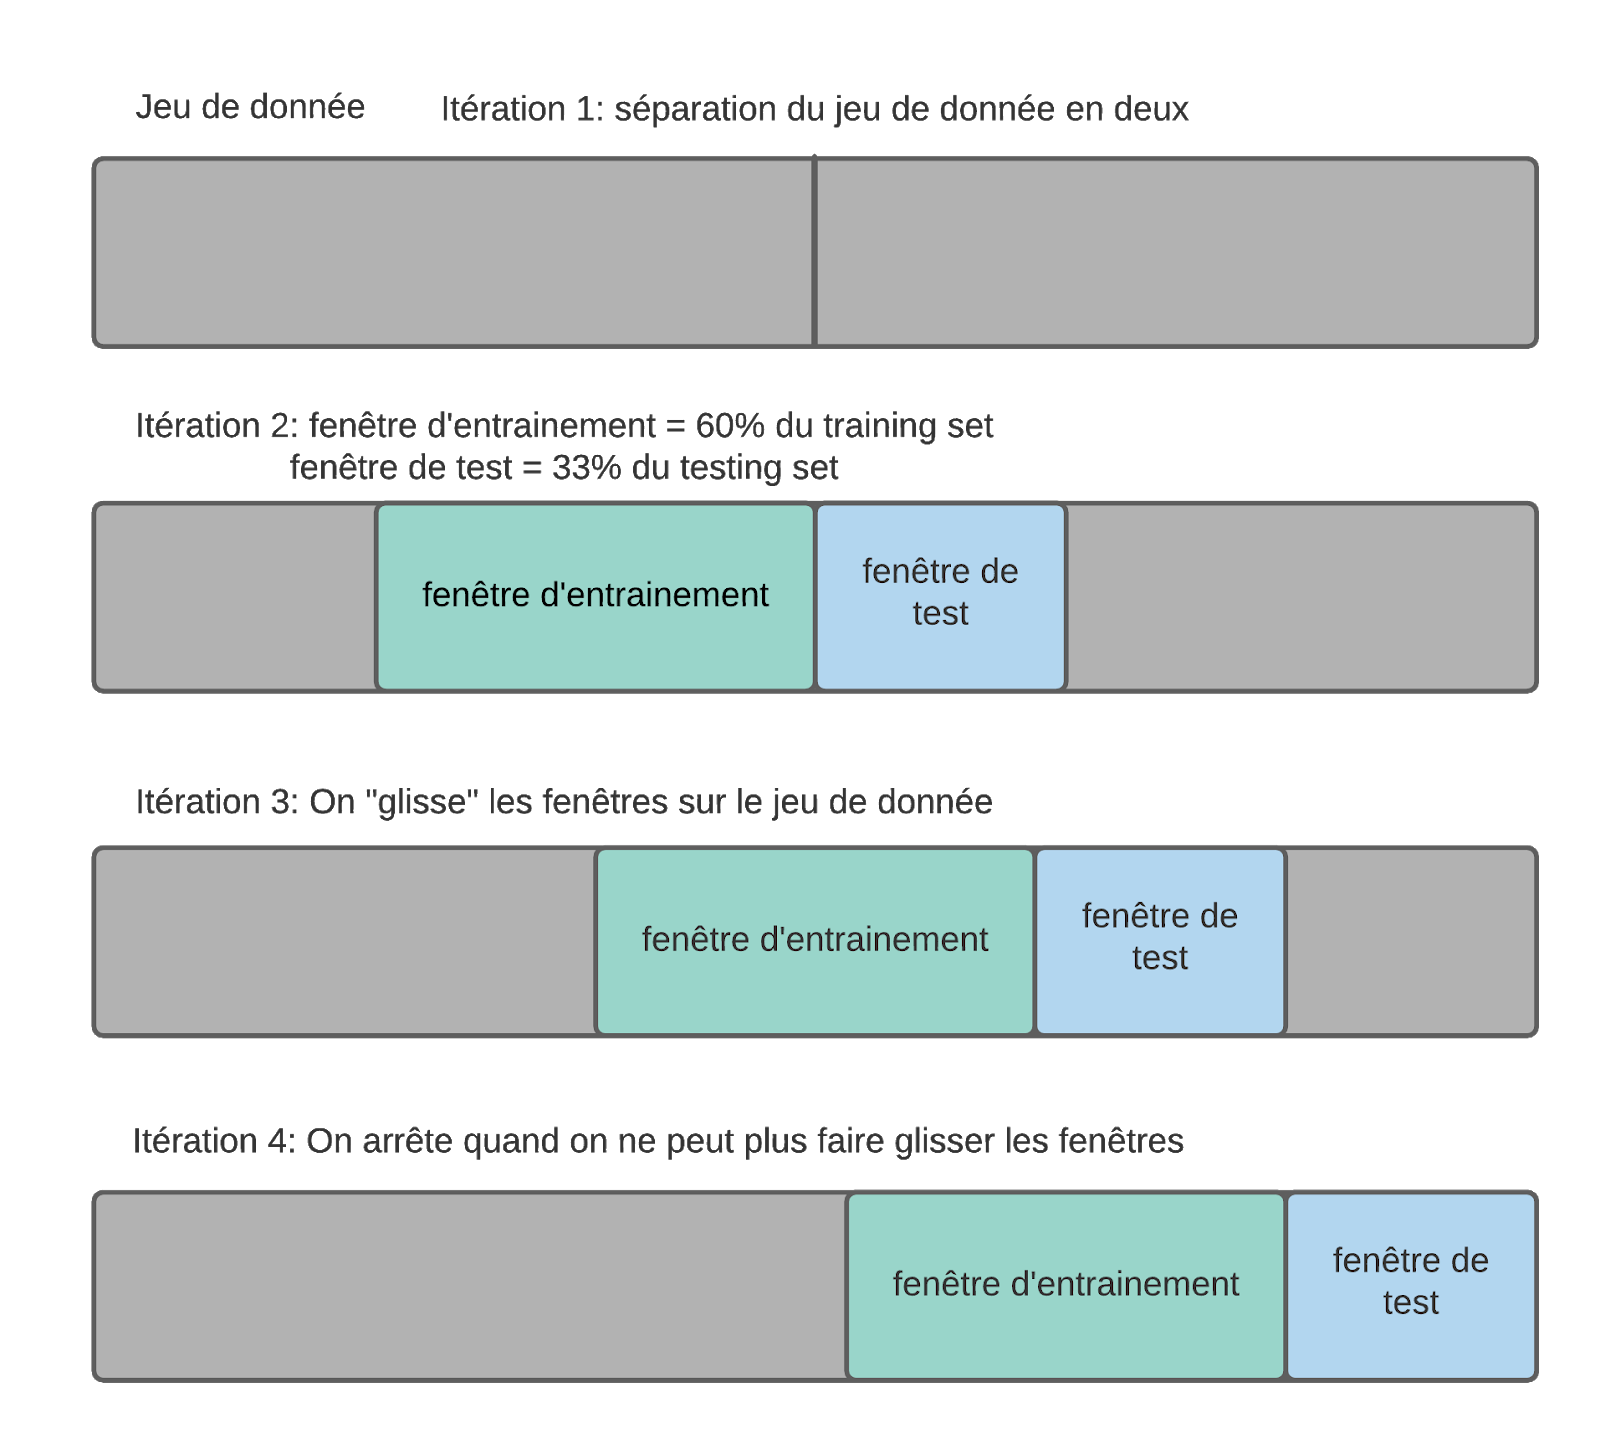
\includegraphics[width=0.8\textwidth]{figures/Sliding_split.png}
\captionof{figure}{Exemple d'apprentissage glissant sur les données}
\label{fig9}
\end{center}

\section{Mesures de performance}
% REM RD: Si tu optes pour la structure en parties
% Je conseille de ne pas faire un chapitre pour "Mesures de performance" mais d'inclure cette
% section dans le chapitre "Évaluation des performances"

% REM RD:
% - Peut-être faire une petite phrase introductive

\subsection{Abstraction}

Une mesure de performance est implémentée au moyen d’une classe abstraite \texttt{PerformanceMeasureBase}. Celle-ci possède:
\begin{easylist}
\ListProperties(Hide=100, Hang=true, Progressive=3ex, Style*=--)
& ~une variable \textit{result} permettant de stocker les résultats de la mesure
& ~une méthode \textit{evaluate} qui renvoie ces résultats
\end{easylist}

Toutes les mesures listées ci-dessous hérite de cette classe abstraite.  

\begin{center}
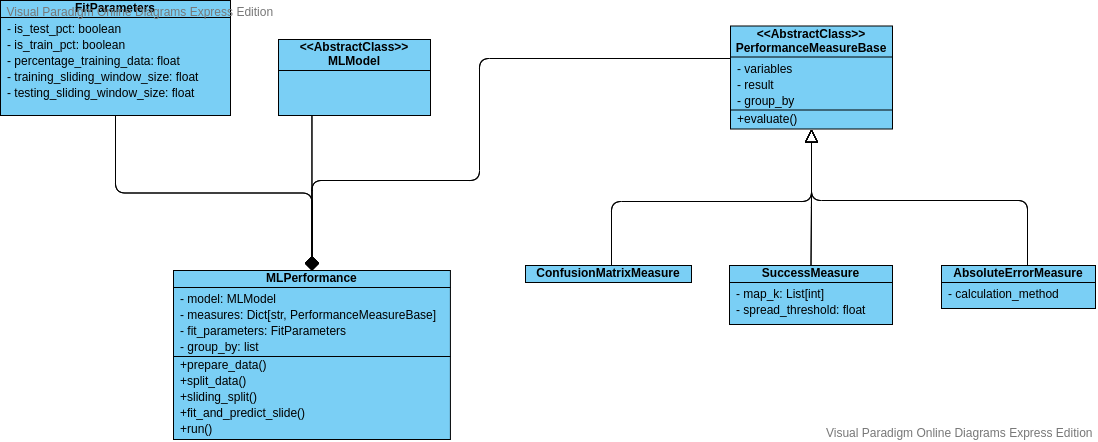
\includegraphics[width=1.1\textwidth]{figures/diagramme_classe_perf.png}
\captionof{figure}{Diagramme de classe du module de performance}
\label{fig5}
\end{center}

\subsection{Mesure de succès}

La première manière la plus intuitive de mesurer la performance d’un modèle dans le cadre d’une classification (i.e. variables cibles catégorielles) est de calculer son taux de succès ou justesse. Le succès est défini comme une bonne prédiction pour la variable cible.

\begin{center}
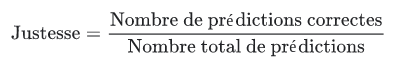
\includegraphics[width=0.6\textwidth]{figures/justesse.png}
\end{center}

Comme illustré sur la Figure \ref{fig5}, cette mesure de succès est implémentée  dans la classe \texttt{SuccessMeasure}. Cette dernière prend deux paramètres:
\begin{easylist}
\ListProperties(Hide=100, Hang=true, Progressive=3ex, Style*=--)
& ~ \textit{map$\_$k}
& ~ \textit{spread$\_$threshold}
\end{easylist}

Le paramètre \textit{map$\_$k} permet de considérer les \textit{k} labels les plus probables suite à la prédiction (i.e. les \textit{k} maximum-a-posteriori). Par défaut, \textit{map$\_$k} est une liste ne contenant que l’entier 1, il n’est considéré alors que le maximum-a-posteriori, mais il est très bien possible d'ajouter différentes valeurs de \textit{k} dans les paramètres pour ainsi considérer les \textit{k} labels les plus probables. On définit donc un succès de la prédiction pour un entier \textit{k} donné du \textit{map$\_$k}, si pour une ligne du jeu de donnée, la valeur à prédire se trouve parmi les \textit{k} labels les plus probables. Logiquement, le taux de succès sur l’ensemble du jeu de donnée de test augmente quand la valeur de \textit{k} croît.

\begin{center}
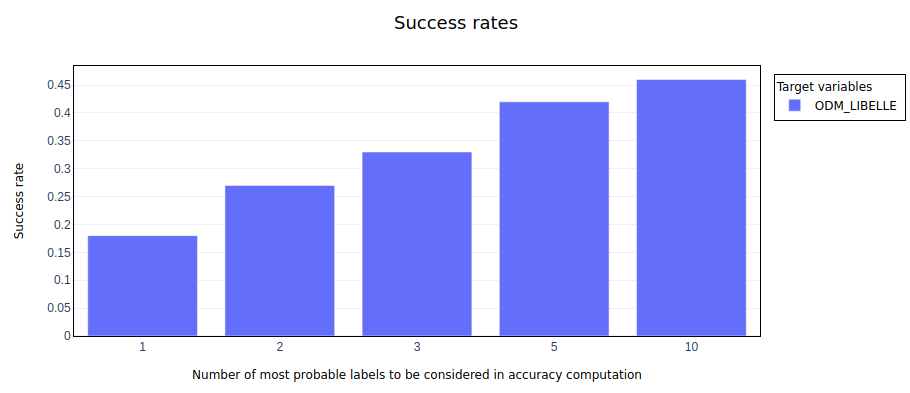
\includegraphics[width=1\textwidth]{figures/rapport_success_rate.png}
\captionof{figure}{Taux de succès pour \textit{map$\_$k} = [1,2,3,5,10] sur le jeu de donnée de la RATP}
\label{fig10}
\end{center}

Le paramètre \textit{spread$\_$threshold} permet quant à lui de définir un seuil d’acceptation d’une prédiction. On redéfinit le succès tel qu’étant donné un entier k du \textit{map$\_$k}, on considère la prédiction comme un succès si la valeur à prédire se trouve parmi les k labels les plus probables et si le pourcentage de marge entre la probabilité du label le plus probable et la probabilité du k-ème label le plus probable est inférieur au \textit{spread$\_$threshold}. Par défaut, le \textit{spread$\_$threshold} est égal à 1, ce qui signifie que l’on acceptera comme étant un succès toute valeur à prédire se trouvant parmi les k labels les plus probables. Ce paramètre permet de ne considérer que les succès où la valeur prédite était un minimum probable. Par exemple, si la valeur à prédire pour l’index 1 de notre jeu de donnée est SOLEIL et que notre fonction \textit{predict} nous renvoie la \texttt{DiscreteDistribution} suivante,

\begin{center}
\begin{tabular}{cccc}
\rowcolor[RGB]{200, 200, 200}index & SOLEIL & PLUIE & NUAGEUX \\
\hline
1 & 0.04 & 0.95 & 0.01

\end{tabular}
\end{center}

il pourrait être absurde de considérer un succès pour une valeur de k égal à 2 car l’écart en pourcentage entre 0.95 et 0.04 est très élevé (=0.9579). C’est pour cela qu’avec un \textit{spread$\_$threshold} = 0.2 par exemple et k = 2, on considérerait un échec de la prédiction car 0.9579 $>$ 0.2.

\texttt{SuccessMeasure} possède aussi un argument result hérité de la classe abstraite \texttt{PerformanceMeasureBase} qui sert à stocker les résultats de la mesure. Dans le cas de \texttt{SuccessMeasure}, \textit{result} est un dictionnaire contenant les trois clés “indep”, “aggreg” et “joint”.
La valeur associée à la clé “indep” correspond aux différents taux de succès pour chaque k appartenant à \textit{map$\_$k} et pour chaque variable cible.
La valeur associée à la clé “aggreg” correspond pour chaque k au nombre moyen de variable cible que l’on prédit à chaque ligne.
La valeur associée à la clé “joint” correspond au taux de bonne prédiction pour chaque combinaison de variables cibles sachant que les autres variables cibles n’ont pas été prédites (par exemple sur la Figure \ref{fig11}, le taux de bonne prédiction de la variable FONCTION$\_$NIV2 sachant que ODM$\_$LIBELLE n’est pas prédit est de 0.5, et le taux de bonne prédiction de la combinaison ODM$\_$LIBELLE - FONCTION$\_$NIV2 sachant que les autres variables, ici aucune, ne sont pas prédites est de 0.27).

\begin{center}
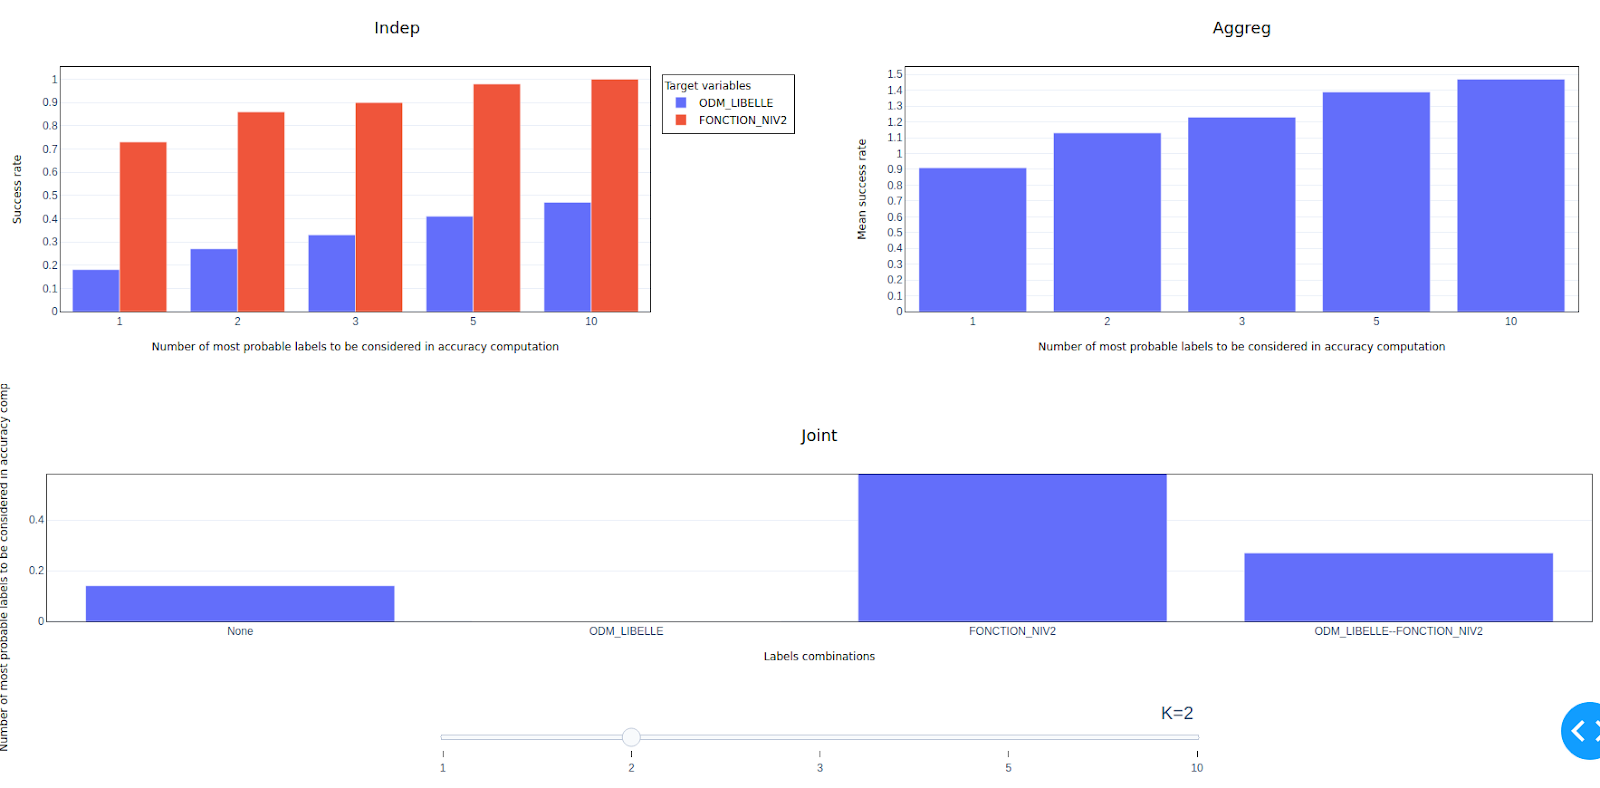
\includegraphics[width=1\textwidth]{figures/visu_success.png}
\captionof{figure}{Visualisations interactive associées à la mesure de succès}
\label{fig11}
\end{center}

\subsection{Matrice de confusion}

Une matrice de confusion est une matrice de taille \textit{n x n} où \textit{n} est le nombre de
labels de la variable cible en question. L'élément d’indice \textit{(i,j)} correspond alors au
nombre de fois que l’on a prédit le \textit{i}-ème label alors que le label à prédire est le
\textit{j}-ième. Les éléments d’indices \textit{(i,i)} correspondent aux cas de bonnes prédictions.

\begin{figure}
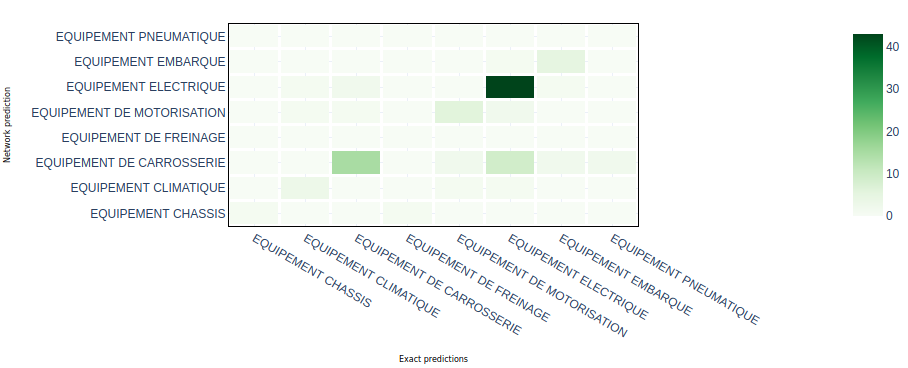
\includegraphics[width=1\textwidth]{figures/confusion_matrix.png}
\captionof{figure}{Exemple de matrice de confusion pour une variable cible à huit labels}
\label{fig12}
\end{figure}

La matrice de confusion peut être assez illisible si on veut afficher des matrices de variables possédant un grand nombre de labels possibles comme c’est le cas pour notre exemple avec la base de données gmao de la RATP dont une des variables cibles possède 1400 labels.

\subsection{Mesure \textit{Absolute Error}}

La mesure d’erreur absolue (\textit{Absolute Error}, en anglais) est définie pour les variables cibles numériques (sous forme de valeurs points ou d’intervalles). On calcule alors l’erreur absolue pour chaque ligne du jeu de donnée de test entre la valeur à prédire et une valeur prédite.
$$\Delta x_{i} = |x_{i}-x^{\star}_{i}|$$
avec $x_{i}$ la valeur de la prédiction i et $x^{\star}_{i}$ la valeur réelle.

% REM RD : Je renouvelle mon conseil d'introduire formellement les notions de EAP et MAP au début du
% chapitre, par exemple là où tu expliques ce qu'est l'apprentissage supervisé.
Le calcul de $x_{i}$ dépend en fait de la méthode de calcul utilisée. La classe comprend donc un paramètre \textit{calculation$\_$method} qui vaut soit \textit{eap} (pour esperance a posteriori), soit \textit{map} (pour maximum a posteriori). Si \textit{calculation$\_$method} = eap, alors $x_{i}$ est égal à la moyenne des labels (qui sont les nombres possibles que peut prendre la variable; on travaille uniquement avec des variables catégorielles) pondérés par les probabilités de la \texttt{DiscreteDistribution} obtenue d’après la fonction \textit{predict}. Ainsi on prend en compte la probabilité de chaque label. Si \textit{calculation$\_$method} = map, on prend $x_{i}$ égal au label le plus probable. Par défaut, \textit{calculation$\_$method} = \textit{eap}.

Si jamais un argument \textit{group$\_$by} a été donné, on calcule également la MAE (\textit{Mean Absolute Error}) sur les données groupées. Dans le cadre du projet, la MAE n’a de sens que pour des données spécifiques au pronostic. 
$$MAE = \frac{1}{n}\sum_{i=1}^{n}|x_{i}-x|=\frac{1}{n}\sum_{i=1}^{n}\Delta x_{i}$$
où $n$ est le nombre de données dans le jeu de test

Le pronostic se distingue du diagnostic dans le sens où l’objectif du diagnostic est de pouvoir prédire le type d’intervention à effectuer sur un système, alors que l’objectif du pronostic est de prédire la RUL (\textit{Remaining Useful Life}) ou temps de vie restant d’un système. 
L’objectif pour un modèle performant est donc de minimiser la MAE afin que la trajectoire prédite de la RUL pour un système donné coïncide au plus avec la trajectoire correspondante des données de test. Ci-dessous, on remarque sans trop de mal que la trajectoire prédite est bien loin de la trajectoire à prédire.

\begin{center}
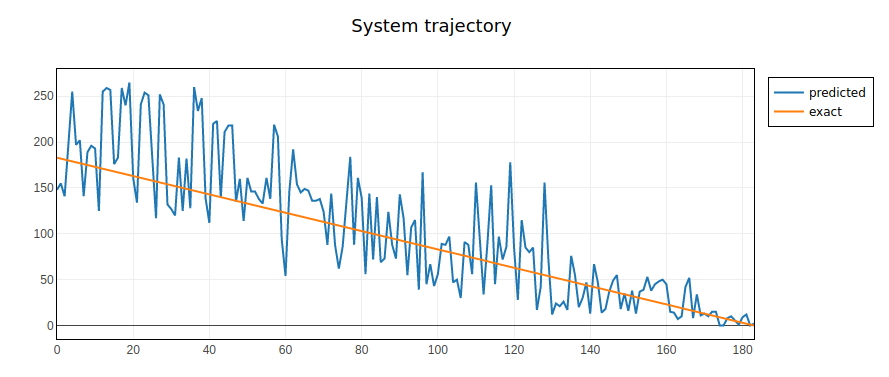
\includegraphics[width=1\textwidth]{figures/system_trajectory.png}
\captionof{figure}{Trajectoire système avec en ordonnée la RUL et en abscisse le temps}
\label{fig13}
\end{center}

\subsection{Création de nouvelles mesures}

L’architecture de la chaîne de traitement permet de facilement implémenter de nouvelles mesures de performance, et ce sera certainement une piste d’ouverture pour la continuité du projet. Un extrait d’un article de Saxena \cite{metrics_saxena} permet de montrer quelles mesures pourraient être implémentées. En voici un exemple avec la \textit{Mean Absolute Percentage Error} (MAPE):
$$MAPE =\frac{1}{n}\sum_{i=1}^{n} \left \lvert \frac{100\Delta x_{i}}{x^{\star}_{i}} \right \rvert $$


\chapter{Visualisations et création d’une application dash}

Les visualisations sont gérées au niveau de chaque composant de la chaîne de traitements en suivant
un formalisme spécifique. Cette architecture
permet alors d'orchestrer efficacement et automatiquement la création de tableaux bords
(\textit{dashboard}) composés de différentes visualisations interactives (e.g. mesures de
performance, comparaison de modèles, etc.). L’application est codée à l’aide de la librairie \texttt{plotly} et plus particulièrement grâce à la fonctionnalité dash de plotly.

À ce jour la plus grosse brique regroupant tous les composants est le module de comparaison de
performances entre plusieurs modèles.

C’est ce qui est présenté dans le schéma Figure \ref{fig15}.


% REM RD: Titre de la figure
\begin{center}
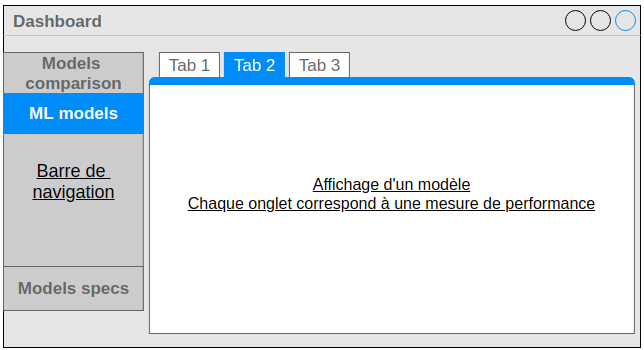
\includegraphics[width=1\textwidth]{figures/schema_app.png}
\captionof{figure}{Schéma du \textit{dashboard}}
\label{fig15}
\end{center}

% REM RD: Je te conseille d'utiliser une liste d'items.
La barre de navigation sur la gauche est décomposée en trois parties: 
\begin{easylist}
\ListProperties(Hide=100, Hang=true, Progressive=3ex, Style*=--)
& ~la première partie compare les modèles selon une mesure donnée
& ~la deuxième affiche les performances de chaque modèle
& ~la troisième partie récapitule les paramètres de chaque modèle.
\end{easylist}

Nous allons voir les différentes visualisations pour chaque partie ci-dessous.

\section{Partie \textit{MODELS COMPARISON}}

% REM RD: Titre de la figure
\begin{center}
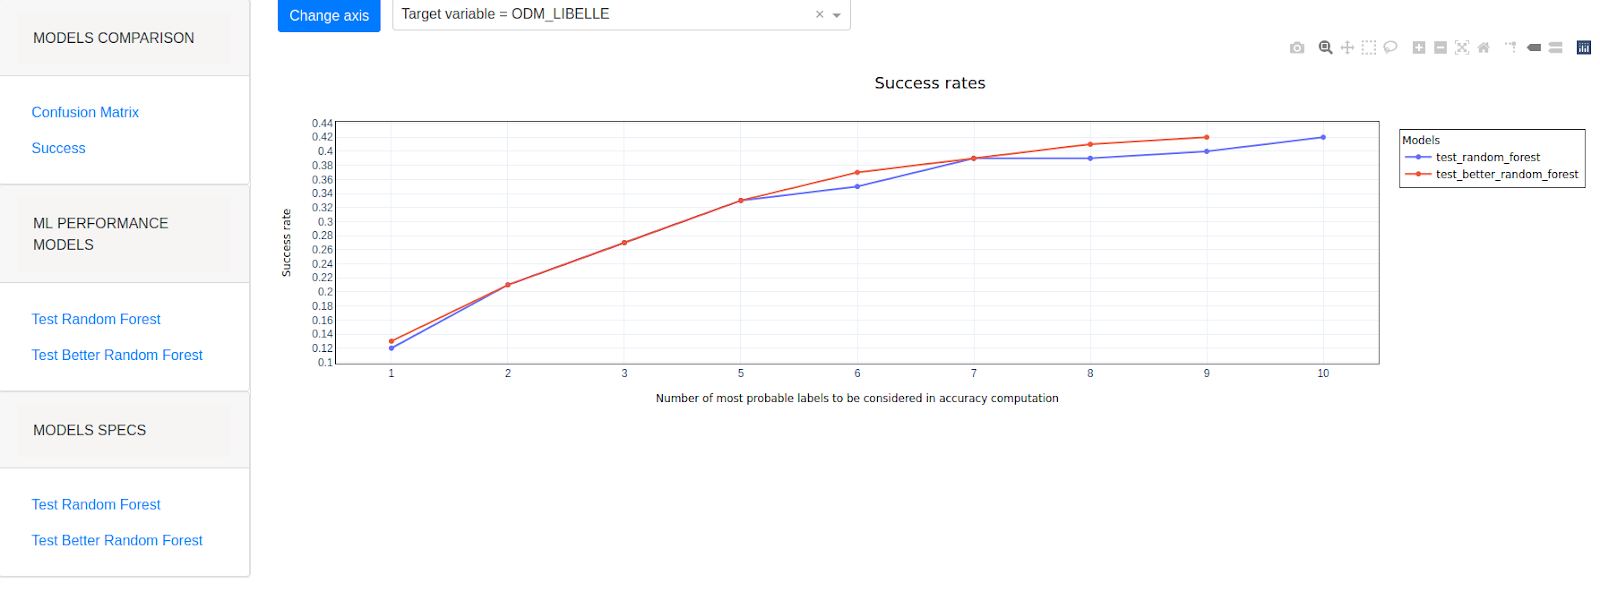
\includegraphics[width=1\textwidth]{figures/app_comparison.png}
\captionof{figure}{Partie \textit{MODELS COMPARISON}}
\label{fig16}
\end{center}

% REM RD: Formulation à améliorer un peu. e.g. La Figure \ref{fig16} présente <bla bla>.
La Figure \ref{fig16} présente l’onglet \textit{Success} de \textit{Models Comparison} affichant le taux de succès de chaque modèle pour une variable cible donnée. Toutes les mesures de performances se trouvent dans la partie \textit{MODELS COMPARISON}. Et il est donc possible de comparer les différents modèles selon la mesure souhaitée.

\section{Partie \textit{ML PERFORMANCE MODELS}}

% REM RD: Titre de la figure ici nous sommes dans l’onglet \textit{Success}.
\begin{center}
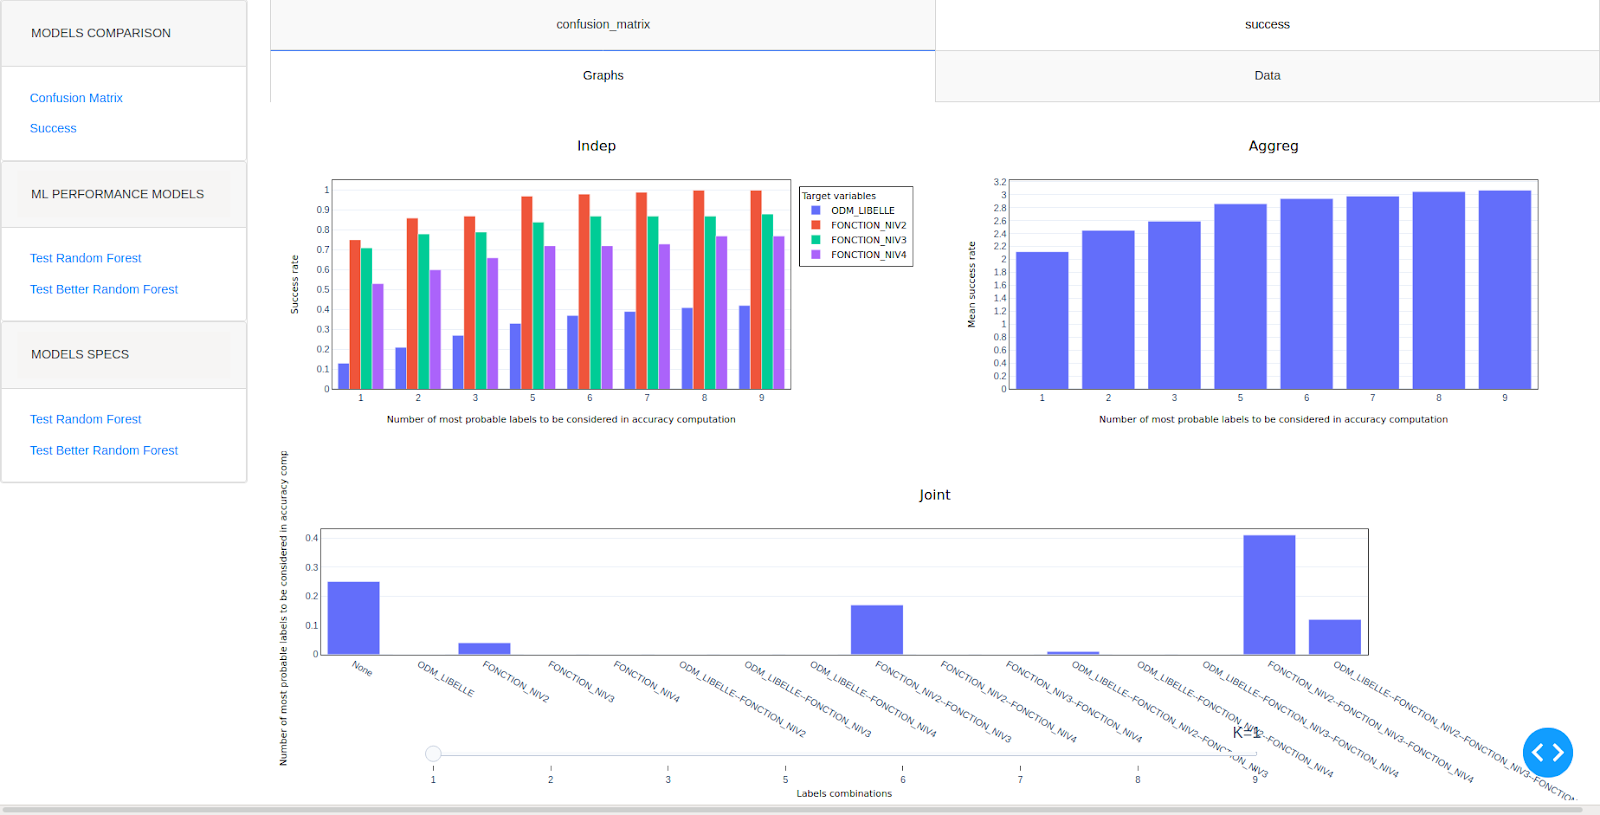
\includegraphics[width=1\textwidth]{figures/app_models.png}
\captionof{figure}{Onglet \textit{Success}, Partie \textit{ML PERFORMANCE MODELS}}
\label{fig17}
\end{center}

% REM RD: peut-être utiliser un autre terme que "brique". Par exemple "espace dédié à l'affichage de
% <tel truc>"
Sur la Figure \ref{fig17} est affichée la visualisation relative à un modèle de la fenêtre
\textit{ML Performance Models}. On retrouve dans la partie supérieure des onglets correspondant à une mesure de performance.
Juste en dessous de cette barre d’onglet se trouve l'espace dédié à l'affichage de la mesure \textit{Success}. Dans cet espace, il y a une autre barre d’onglet avec d’un côté les différents graphes (Figure \ref{fig17}) et de l’autre les données du jeu de test avec les prédictions probabilistes (Figure \ref{fig18}).

% REM RD: Titre de la figure
\begin{figure}
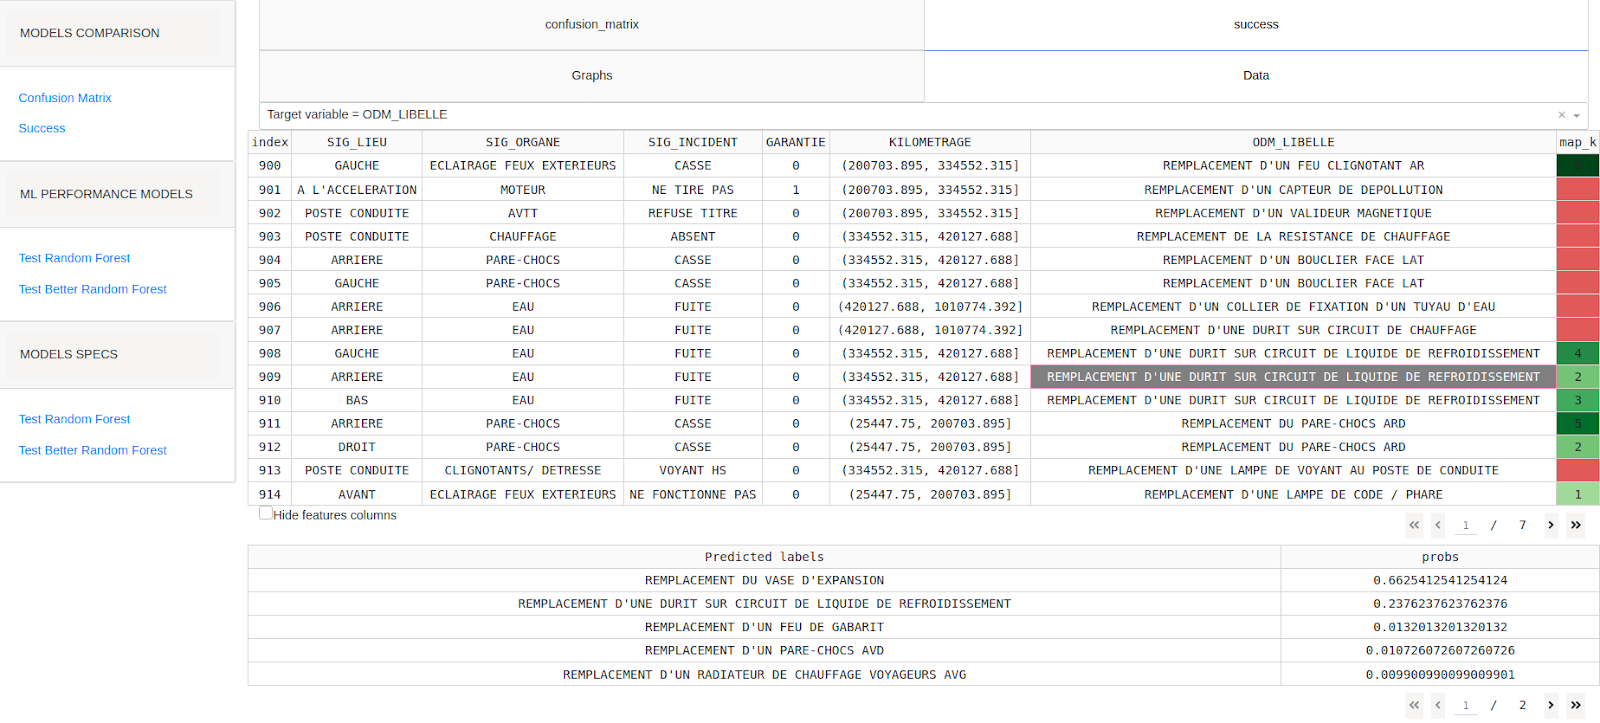
\includegraphics[width=1\textwidth]{figures/app_models_table.png}
\captionof{figure}{Affichage des données}
\label{fig18}
\end{figure}

\section{Partie \textit{MODELS SPECS}}

Enfin comme montré sur la Figure \ref{fig19}, on affiche les différents paramètres du modèle sélectionné dans la fenêtre \textit{Models Specs}.

\begin{center}
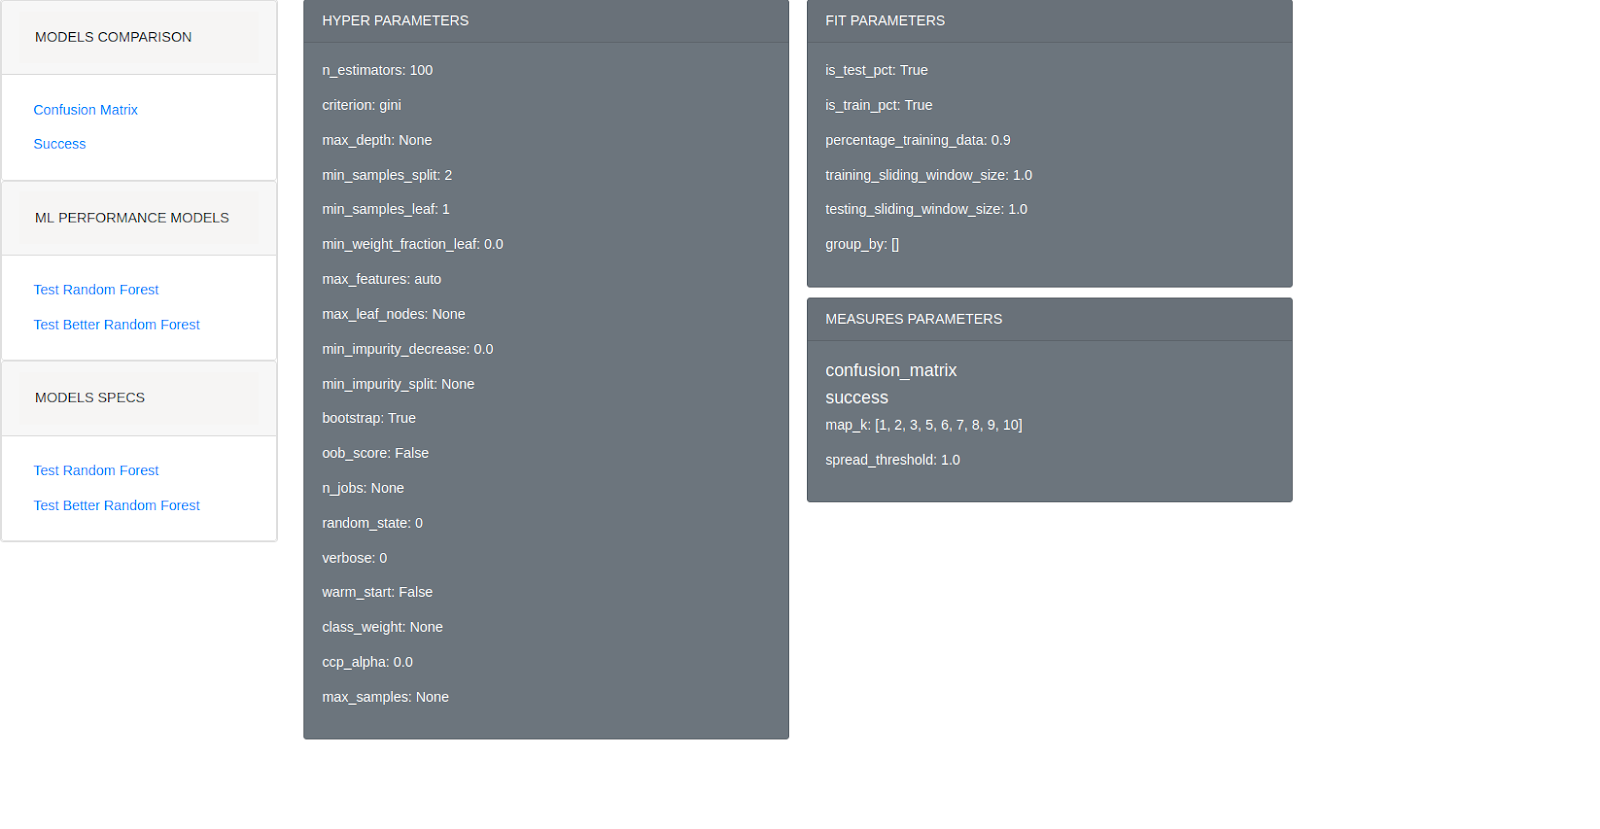
\includegraphics[width=1\textwidth]{figures/app_specs.png}
\captionof{figure}{Partie \textit{MODELS SPECS}}
\label{fig19}
\end{center}

\chapter{Apports du projet et évolutions}

\section{Compétences mobilisées}

En termes de connaissances techniques, mes compétences en programmation objet et en représentation UML m’ont permis de penser efficacement à la structure du projet et à la modélisation de la chaîne de traitement. Par ailleurs, les notions de machine learning vues à l’école m’ont permis de me lancer beaucoup plus rapidement dans la réalisation du code.

Concernant les soft skills, le travail en autonomie a bien sûr été prédominant dans un contexte de télétravail imposé par la crise sanitaire de la COVID-19.

\section{Difficultés rencontrées}

Les difficultées du projet résident surtout dans la compréhension des différentes librairies python, que ce soit pydantic, pandas ou plotly. Par exemple, la structure de l’application requiert qu’on puisse fabriquer des composants graphiques “à la volée”. Or il y avait un problème dans la lecture des callbacks (au moment d’exécuter ces éléments “à la volée” ) pour rendre les visualisations interactives. Ce point n’était pas abordé dans la documentation de dash et il a fallu que je teste plusieurs versions différentes avant de comprendre comment résoudre ce problème.

\section{Compétences acquises}

Les progrès se sont surtout fait sur la partie technique, que ce soit pour l'organisation du code, l'amélioration des \textit{coding skills}, la manipulation des données, la compréhension des modèles de \textit{machine learning}. De plus, le stage a été l'occasion de monter en compétence sur le logiciel de contrôle de version \textbf{git}.

\section{Évolution du projet}

La chaîne peut encore être largement améliorée. Il est tout d’abord possible de compléter les modules déjà existant, en ajoutant de nouvelles mesures de performances, de nouveaux algorithmes de sélection de variables, etc. Ensuite un des enjeux futures est de pouvoir créer un module permettant d’optimiser les paramètres des différents modèles pour obtenir des performances optimales de prédictions. Enfin il reste à styliser et compléter les visualisations déjà existantes.

Une autre évolution du projet évoquée est la possibilité de mettre le projet en open source. Le fort pouvoir collaboratif de la communauté pourrait ainsi permettre au projet de prospérer et d’être utiliser par un grand nombre de personnes.

\section{Evolution personnelle}

La chaîne de traitement a désormais une base solide pour permettre la bonne continuation des développements. Ce projet m’a conforté dans mon idée de poursuivre dans le domaine de la R\&D. \cite{neapolitan_learning_2007}


\singlespacing

% the back matter
\clearpage
\bibliography{BN}
\addcontentsline{toc}{chapter}{References}
\bibliographystyle{plainnat}

\end{document}
